\documentclass[a4paper,12pt,hidelinks]{report}

%%Pacchetti utili anche se non necessari

\usepackage{amsfonts}
\usepackage{amsmath}
\usepackage{latexsym}
\usepackage{tabularx}
\usepackage[italian]{babel}
\usepackage[bookmarks=true]{hyperref}
\usepackage{url}
% \usepackage{subfigure}
\usepackage{epstopdf}
\usepackage[utf8]{inputenc}
% \usepackage[utf8x]{inputenc}
\usepackage{listings}
\usepackage{graphicx}
%-------------------------------------------

% \title{Progettazione sito web\\ ''B\&B La Vecchia Posta''}
% \author{Daniele Di Pompeo \\mat. 226766}
% \annoaccademico{2013-2014}
\begin{document}
\begin{titlepage}
  \begin{center}
  % Upper part of the page
    
\includegraphics[width=0.5\textwidth,keepaspectratio=true]{img/logo}\\[1cm]    
    \textsc{\LARGE Specifiche dei requisiti}\\[0.6cm]
    \textsc{\LARGE  sito: ``B\&B La Vecchia Posta''}\\ [2.0cm]

  % Author and supervisor
    \begin{minipage}{0.8\textwidth}
      \begin{flushleft} \large
	\emph{Autore:} Daniele Di Pompeo \\[0.5cm]
	\emph{Versione documento: 1.0}\\[0.5cm]
	\emph{Data emissione del documento: \today}\\[0.5cm]
      \end{flushleft}
    \end{minipage}
  \end{center}
\end{titlepage}

\tableofcontents

%----------------------------------------------------
\begin{abstract}
  In questo documento verranno descritti nel dettaglio tutti i requisiti funzionali e non funzionali individuati per la realizzazione del sito web del B\&B La Vecchia Posta.
  Per la realizzazione del nuovo sito web sono state utilizzate le informazioni sul traffico dati utilizzando ``google analytics''. Sono stati presi in visione i siti web di altre strutture
  locali e nazionali per rendere la versione 2.0 del sito del B\&B La Vecchia Posta utilizzando tutte le nuove tecniche del web 2.0.
  \par Nella prima parte di questo documento si riporta una descrizione dell'attività del committente ponendo l'attenzione sui dati statici raccolti.
  \par Nella seconda parte vengono descritti in maniera puntuale i requisiti funzionali per la realizzazione del nuovo sito web.
  \par Come framework di sviluppo verrà utilizzato ``beContent'' tool sviluppato dall'università dell'Aquila, del quale il sottoscritto è uno sviluppatore.
  \par Nella stesura di questo documento si fa presente al lettore che in alcune sezioni la figura del committente e del progettista vengono specificatamente separate mentre in altre si tende a 
  descriverle come un'unica persona. Questo perchè in alcuni punti del documento è risultato conveniente separare le due figure nell'ipotesi di un cambiamento futuro, nel quale il progettista 
  non è anche il committente.
\end{abstract}

\chapter{Generalità}

\section{Il Committente}
  Il B\&B La Vecchia Posta, inaugurato nell'Agosto del 2010 è situtato in Via Amiternum n 6 nel comune di Cagnano Amiterno, a pochi chilometri dal centro della città di L'Aquila.
  Offre ai suoi clienti 6 spaziose camere tutte con bagno privato, ampio spazio verde di proprietà garantendo ai suoi clienti il massimo confort e relax. 
  Si riporta una veduta aerea dell'area del B\&B per far rendere conto al lettore la posizione geografica e la conformazione dello spazio (fig.\ref{fig:bbArea}). 

  \begin{figure}[h!]%
    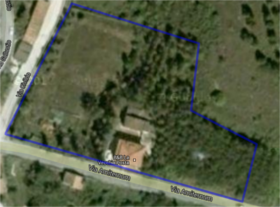
\includegraphics[width=0.6\textwidth,keepaspectratio=true]{img/bbArea1}
    \centering
    \caption{veduta area del B\&B La Vecchia Posta}%
    \label{fig:bbArea}%
  \end{figure}
  Il B\&B è a conduzione familiare, il titolare, l'autore di questo documento, è aiutato dai genitori Emanuela e Nando, incuriositi nel conoscere nuove persone per imparare usi e costumi di diversi luoghi.

\section{Situazione attuale}
  Il B\&B La Vecchia Posta risulta essere titolare di un dominio web dall'URL www.vecchiaposta.it, al momento non sono stati previsti alias. 
  \par Il sito web è stato realizzato nel 2010 dalla Fermenti Grafici, web agency aquilana, che a titolo di amicizia ha realizzato
  il comparto grafico (logo, foto, template) ed ha fornito gratuitamente e momentaneamente l'hosting.
  Ad oggi il sito web risulta essere completamente gestito dal sottoscritto ed è hostato dalla web farm ARUBA.
  \par Sin dalla sua prima versione il sito web del B\&B è stato realizzato utilizzando WordPress, uno dei più famosi CMS nel mondo del web e sono stati installati alcuni plug-in per fornire al sito alcune 
  funzionalità di cui il committente aveva bisogno.
  \par Dall'analisi dei dati raccolti il sottoscritto si è reso conto che molta della pubblicità programmata su internet, tramite il servizio ``google adword'', non portava ai risultati attesi,
  quindi è sorta la neccessità di aggiornare il sito web attuale.

\subsection{Aspetti rilevanti del sito}
  Da interviste effettuate sui clienti del B\&B risulta essere di gradevole impatto il sito, grazie ad una grafica curata minuziosamente.
  Sempre ascoltando i parari di terzi il sito web risulta essere di gradevole navigazione offrendo informazioni dettagliate per le singole pagine.

\subsection{Principali pregi}
  L'intero sito web non ha oggetti in flash, che renderebbero il sito non navigabile dadispositivi mobile.
  \par La home page effettua 86 HTTP Request per un peso complessivo di circa 60Kb scaricabili in circa 3 secondi con una connessione a banda larga di velocità media (4Mb)
  \par La struttura dell'intero sito è sempre coerente fornendo uno spazio per l'immagine principale della pagina, che può anche essere uno slider, 
  e dello spazio binanco per il testo rendendo la lettura gradevole non affaticando gli occhi del lettore.

\subsection{Principali difetti}
  I principali difetti sono legati dalla difficoltà nel raggiungere il collegamento per effettuare una richiesta di prenotazione, accessibile 
  solamente tramite la barra di nabigazione o tramite il link nascosto dietro il testo dell'ultimo articolo inserito, che nel nostro caso sono le ultime news.
  \par Questo è visibile anche dai dati statistici raccolti da google analytics che mostrano come l'utente navighi nel sito 
  poco meno di 2 minuti e lo abbandona prima di inviare una richiesta di prenotazione. Evidente dal fatto che il link prenota non risulta mai essere cliccato.
  \begin{figure}[h!]%
    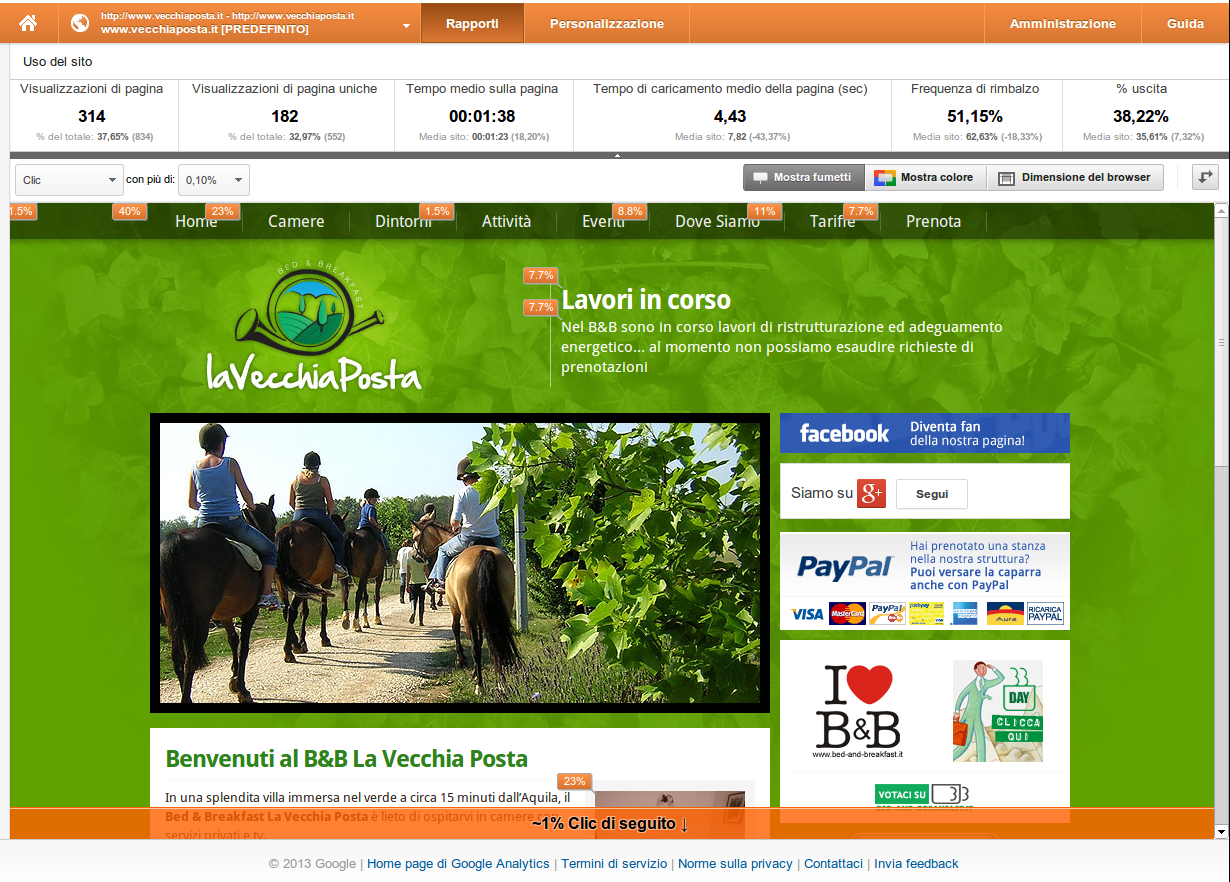
\includegraphics[width=0.95\textwidth,keepaspectratio=true]{img/googleAnalyticsDoc1}
    \centering
    \caption{Dati Google Analitycs Home Page}%
    \label{fig:googleHomePage}%
  \end{figure}
  Dall'immagine fig.\ref{fig:googleHomePage} risulta evidente che la barra di navigazione posta sopra il logo rende difficoltosa all'utente medio comprendere quale sia il vero link alla home page.
  Si notano alcuni click sullo spazio negativo della barra di navigazione (più del 40\% degli utenti).
  \par Nella sezione ``Appendice B'' vengono riportare altre immagini e dettagli a supporto degli aspetti negativi della versione attuale 
  del sito web.
  \par Non permette la modifica della grandezza del font, non permettendo una facile navigazione a persone ipovedenti. Analizzando il tema del sito 
  con il serivizio offerto dal sito \url{http://colorfilter.wickline.org/} risulta perdere completamente l'effetto desiderato mostrandosi piatto 
  e privo di effetti grafici. 

\section{Obiettivi generali del nuovo sito}
  La nuova versione del sito web dovrà eliminare queste problematiche, invogliando gli utenti ad inviare più richieste di prenotazioni inserendo nella parte ``sopra la piega'' 
  un link al ``form'' di prenotazione di prenotazione.
  \par Per il comparto grafico si è scelta di comprare un tema html dal sito \url{www.themeForest.com}, con le caratteristiche grafiche richieste.
  \\ Il nuovo sito inoltre, nella versione base dovrà fornire le informazioni ad oggi presenti migliorando la navigabilità spostando la barra di navigazione al di sotto del logo del B\&B, 
  aspetto grafico maggiormento utilizzato.
  \par L'home page del sito dovrà restare leggera e non dovrà prevedere nessuna funzionalità in flash, che la renderebbe inaccessibile dai dispositivi mobile.
  L'intento è di fornire ``\textit{sopra la piega}`` tutte le informazioni utili come:
  \begin{itemize}
    \item collegamento all'home page al click sul logo
    \item barra di navigazione al di sotto del logo
    \item slider di immagini
    \item form per la richiesta di disponibilità
    \item preview dell'offerta attiva
  \end{itemize}
  \par Inoltre il nuovo sito dovrà essere ''responsive'' garantendo la completa compatibilità con i maggiori device che ad oggi accedono ad internet.
  \\In particolare:
  \begin{itemize}
    \item 1200px Desktop
    \item 1024px iPad landscape and netbook
    \item 768px 7inch tablet
    \item 368px mobile phone
  \end{itemize}
  Prendendo come risoluzione base 1200px essendo circa il 90\% degli utenti ad utilizzarla \footnote{Fonte \url{http://www.w3schools.com/browsers/browsers_display.asp}}
  ed inoltre facendo attenzione alla compatibilità fra i differenti browser (chrome, firefox, safari, explorer ed opera).

\section{Utenti}
  Dall'analisi effettuata risultano essere stati individuati tre categorie di utenti:
  \begin{itemize}
    \item L'amministratore
    \item L'utente occasionale (utente che raggiunge il sitoweb involontariamente) (aka \textit{Utente})
    \item Il cliente (navigatore di internet che effettua una richiesta di prenotazione)
  \end{itemize}
  \begin{center}
    \begin{tabular}{||m{3cm}||m{4cm}|m{1,5cm}||m{4cm}|m{1,5cm}||}
      \hline
	\textbf{Categoria di utenti} & \textbf{Bisogni principali degli utenti in relazione al sito} & Priorità & \textbf{Obiettivi del committente} & Priorità \\
      \hline
	Amministratore & mantenere aggiornarnate le informazioni presenti sul sito & alta & fornire all'amministratore le informazioni aggiornate da inserire nel sito web & alta\\
      \hline
	Utente & reperire le informazioni di contatto, prendere visione della struttura
	      & alta, alta
	      & impressionare l'utente casuale invogliando ad effettuare una prenotazione,  & alta\\
      \hline  
	Cliente & reperire informazioni di contatto, visionare il tariffario, effettuare una richiesta di prenotazione & alta, media, alta & mantere ottimi rapporti con
	il cliente abitudinario, invogliare il ``passaparola'' dei clienti & alta, alta\\
      \hline
    \end{tabular}
  \end{center}
  \subsection{Profilo degli utenti}
    \begin{itemize}
    \item \textbf{Cliente}: sono i navigatori di internet che cercando una destinazione per le proprie vacanze si sono imbattuti sul sito web della struttura e hanno la volotà di inviare 
    una richiesta di disponibilità. Rientrano in questa categoria di utenza anche i clienti ``storici'' del B\&B avendo già soggiornato nella struttura in un'altra occasione.
    \item \textbf{Utente}: sono i navigatori di internet definiti come i visitatori di rimbalzo, ovvero quegli utenti di internet che non volendo sono giunti sul sito internet del B\&B. 
    Su questi utenti che il titolare vorrebbe invogliare a fare una richiesta di disponibilità.
    \end{itemize}

\section{Scenari d'uso}
  \par
  \begin{itemize}
  \item \textbf{Cliente}: Michela è una gentile signora che lavora presso un'agenzia per il turismo nazionale e con la voglia di scoprire le bellezze naturalistiche e magari trovare
  un nuovo cliente per il suo impiego decide di prenotare una vacanza di qualche giorno in un B\&B del parco nazionale del gran sasso. Navigando in internet e utilizzando i portali 
  più famosi del settore è riuscita a navigare sul sito del B\&B La Vecchia Posta. Attirata dalle foto effettua una prenotazione. Da allora Michela trascorre le sue vacanze estive nel 
  B\&B La Vecchia Posta.
  
  \item \textbf{Utente}: Antonietta ragazza di 23 anni studentessa di filosofia a Bologna non è la classica ragazza che gli amici eticheterebbero come ``tecnologica''. Infatti ama utilizzare
  il suo vecchio telefono nokia con il tastierino numerico e schermo non touch. 
  \par Navigando in internet per una ricerca universitaria inizia a seguire una serie di link pubblicitari accattivanti
  per prenotare le proprie vacanze a prezzi super stracciati. Non essendo un'abile navigatrice di internet non si rende facilemnte conto di ciò che sta facendo, ma cliccando su un link piuttosto che su un altro
  finalmente la sua attenzione viene colpita dal sito del B\&B La Vecchia Posta. Recupera facilmente i recapiti telefonici effettua una chiamata al B\&B e prenota la sua vacanza.
  \end{itemize}

\section{Posizionamento competitivo}
  Particolare attenzione verrà posta nel posizionamento competitivo il sito web della struttura.
  \\Per ottenere un risutlato di pregio sono stati analizzati i siti web di altre strutture locali ma anche di strutture nazionali, delle maggiori località turistiche, 
  per catturare quelle funzionalità che potevano sfuggire ma che risultano essere utili.
  \par I siti web locali analizzati sono stati:
  \begin{itemize}
    \item B\&B Camaga
    \item B\&B Oasi nel Vetoio
    \item B\&B Grace
  \end{itemize}
  mentre per i siti extra-regione sono stati analizzati:
  \begin{itemize}
    \item Il giglio binaco (Sorrento)
    \item Soggiorno Pezzati (Firenze)
    \item Il Melograno (Muro Leccese)
  \end{itemize}
  Per l'analisi dettagliata sui siti web analizzati si rimanda alla sezione ``Appendice A''.
  \par Per il nuovo sito si intende migliorare l'indicizzazione sui principali motori di ricerca (google, bing, yahoo) posizionandolo nei primissimi posti 
  seguendo le direttive imposte dai motori di ricerca.

\chapter{Requisiti del sito}

\section{Requisiti di architettura}
  \subsection{Architettura informativa}
   \begin{itemize}
    \item Home
      \begin{itemize}
	\item Camere
	  \begin{itemize}
	    \item Singola
	    \item Doppia
	    \item Tripla
	    \item Quadrupla
	  \end{itemize}
	\item Eventi
	  \begin{itemize}
	    \item Perdonanza Celistiniana
	    \item Festa del Cioccolato
	    \item Sagre e Feste
	  \end{itemize}
	\item Attività
	  \begin{itemize}
	    \item Ippovia del Gran Sassi
	    \item L'anello del Lago di Campotosto
	    \item Da Cagnano al Gran Sasso
	  \end{itemize}
	\item Dintorni
	  \begin{itemize}
	    \item L'Aquila
	    \item Amatrice
	    \item Parco Nazionale del Gran Sasso
	    \item Lago di Campotosto
	    \item Campo Imperatore
	    \item Campo Felice
	  \end{itemize}
	\item Dove Siamo
      \end{itemize}
    \end{itemize}

  \subsection{Navigazione}
    Per quanto riguarda la navigazione del sito sarà necessario organizzare una barra di navigazione orizzontale che permetta all'utente di spostarsi facilmente da una sezione di primo livello
    ad un'altra. La barra di navigazione di primo livello si è deciso di posizionarla al di sotto del header, che contiene il logo dell'azienda e la preview dell'offerta attiva. 
    Al di sopra del logo si pensa di sistemare i collegamenti alle pagine social, link che vengono utilizzati in minor modo.
    Inoltre sempre nella parte alta della pagina viene utilizzato il classico ``marker'' utilizzato nelle mappe come scorciatoia per mostrare la mappa velocemente, 
    un pulsante per effettuare una rihciesta di prenotazione e i bottoni per la gestione della grandezza dei font.
    \par Per le sezioni di secondo livello si pensa di utilizzare una barra di navigazione verticale per permettere all'utente di spostarsi agevolmente nelle varie sezioni interne senza
    perdersi nei vari link del sito. Il menu di secondo livello verrà posizionato nella sidebar di destra, appena sotto lo slider, suddividendo lo spazio della pagina in un 70\% destinato 
    ai contenuti ed un 30\% destinato al menu di secondo livello.
    \par Si riporta uno schema della gabbia logica per l'home page del sito. Le altre pagine manterranno una struttura simile all'home page garantendo alta la coesione tra i contenuti.
    \\Nella fig.\ref{fig:gabbiaLogica} viene riportata la struttura dell'intero sito e non solo della home page mostrando anche 
    il posizionamento della barra di navigazione di secondo livello ove presente.
    \begin{figure}[h!]%
      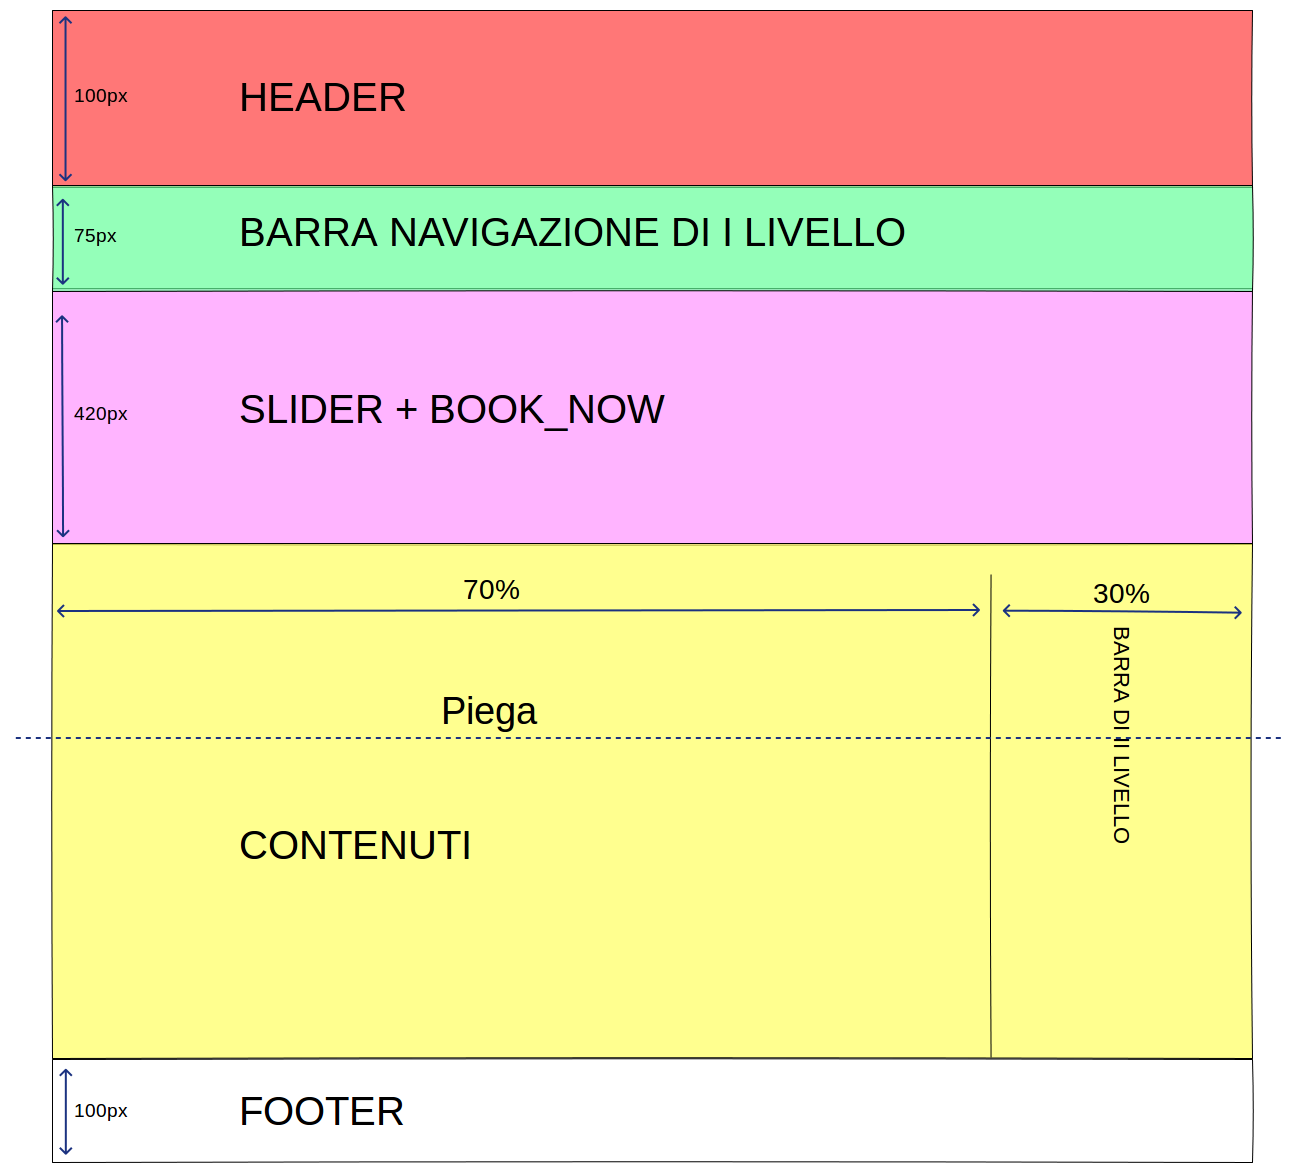
\includegraphics[width=0.95\textwidth,keepaspectratio=true]{img/gabbiaLogica}
      \centering
      \caption{Gabbia logica}%
      \label{fig:gabbiaLogica}%
    \end{figure}
  \newpage
  
\section{Requisiti di comunicazione}
  \subsection{Identità di marca, tono e stile della comunicazione}
    Semplicità, eleganza e calore sono le caratteristiche che il comparto grafico del sito dovrà rispettare essendo le caratteristiche dell'azienda. 
    Si è scelto una palette di colori che richiami il logo dell'azienda mantenendo uno stile aggraziato che richiami anche i colori della terra. I colori dominanti per il sito
    sono il verde e il marrone. Nella parte sopra la piega oltre al form per la richiesta di disponibilità si è deciso di insere uno slider in modo da ottenere una home page
    stile vetrina, metodo che attualmente è più in voga nei siti internet delle aziende nel campo del turismo. Nella sezione sotto la piega sono stati collocati invece i contenuti multimediali
    che risultano essere di minore rilevanza al fine di ottenere una richiesta di prenotazione.

  \subsection{Grafica e multimedialità}
    Per il comparto grafico si pensato di prendere come risoluizione base del sito i 1200px di larghezza, essendo la risoluizione di maggiore utilizzo\footnote{Dati di \url{www.w3schools.com}}.
    Non sono quindi previsti scroll orizzontali ma solo verticali, mantenendo \textit{sopra la piega} tutte le informazioni principali e la barra di navigazione primaria. Per mantenere
    il sito al passo con i tempi si è deciso di renderlo anche responsive, prevedendone una versione per smartphone e tablet oltre che per desktop.
  \subsection{Lingua e localizzazione}
    Per lo sviluppo del nuova versione del sito, si è scelto di utilizzare il framework beContent, ciò ci permette in automatico la scelta della lingua preferita dall'utente, potendo eliminare i bottoni per la 
    scelta della lingua del sito. 

\section{Requisiti funzionali}
  \subsection{Casi d'uso}
    Per la realizzazione del nuovo sito internet sono stati individuati, in prima analisi, i seguenti casi d'uso per i singoli attori. Si fa presente che i seguenti casi d'uso verranno
    riportati sia in forma non dettagliata che dettagliata e che essendo i casi d'uso analizzati nella fase di indagine, potranno subire delle modifiche nelle fasi successive dello sviluppo.
    \begin{itemize}
    \item Amministratore:
      \begin{enumerate}
	\item UC1: Inserire contenuti
	\item UC2: Aggiornare il sistema
	\item UC3: Mantenere frunzionante il sistema
      \end{enumerate}
    \item Cliente: 
      \begin{enumerate}
	\item UC4: Visualizzare le informazioni di contatto
      \end{enumerate}
    \item Utente: 
      \begin{enumerate}
	\item UC5: Effettuare una richiesta di prenotazione
      \end{enumerate}
    \end{itemize}
    Si rimanda il lettore all'appendice C per la lettura dei casi d'uso in forma dettagliata.

  \subsection{Base di dati}
    La nuova versione del sito internet, non utilizzerà la vecchia base dati, ma sarà sviluppata una nuova base di dati rispettando le esigenze del nuovo framework di sviluppo.
    \par Nella nuova base di dati verranno memorizzati tutte le informazioni necessarie al funzionamento di beContent, come la password di amministratore e di tutti gli utenti che devono
    interagire con lo stesso (attualmente l'amministratore di sistema è anche il committente quindi un solo utente avrà i diritti per l'accesso nell'area di backend del framework).
    Verranno inoltre memorizzati i contenuti delle pagine interne (testo, link, file multimediali).

  \subsection{Sicurezza e privacy}
    Nella versione 1.0 del nuovo sito non è previsto il mantenimento delle informazioni dei clienti su database, ma solamente l'invio tramite email dei dati utili alla prenotazione di una camera.
    All'utente sarà comuque richiesto esplicitamente di accettare le codizioni sull'utilizzo dei propri dati in conformità con la normativa art. 13 del d.lgs. 196/2003.

\section{Requisiti di contenuto}
  Essendo l'amministratore l'unica figura responsabile ad utilizzare il framework, sarà suo compito inserire, modificare ed eliminare i contenuti multimediali del sito.
  \par Le sezioni in lingua straniera (inglese, spagnolo) saranno redatte dal sottoscritto coadiuvato da Antonietta, laureata in lingue straniere (inglese e spagnolo).
  \\Le due lingue straniere scelte sono dovute dal fatto che molte delle visite al sito internet provengono oltre che dall'Italia, dagli Stati Uniti dall'Inghilterra e dal Brasile 
  come viene mostrato dalla figura \ref{fig:googleAnalyticsPaesi} nella sezione ``Appendice B''.

\section{Requisiti di gestione}

  \subsection{Infrastruttura per l'esercizio del sito}
    Si presuppone di hostare il nuovo sito internet su una web farm che offra anche servizio SMTP per l'invio di email. 
    Il B\&B La Vecchia Posta risulta essere titolare di un dominio internet \url{www.vecchiaposta.it},
    non si ha la necessità di registrare alias e altri domini, almeno per il momento.
    \par Il B\&B ha inoltre una casella di posta elettronica utilizzata per la ricezione delle richieste di prenotazioni e per le risposte ai clienti. 
    Risulta utile utilizzare i servizi di Antivirus, AntiSpamm che la web farm offre per rendere più confortevole l'utilizzo della mail, eliminando i 
    messaggi indesiderati.
    
  \subsection{Gestione dei sistemi}
    Il sitema sarà affidato in outsourcing, ed è stato scelto come gestore esterno la compagnia Aruba, tra le web farm più in voga al momento.
    \par Nella fase iniziale non è venuta alla luce l'esigenza di richiedere al gestore caratteristiche particolari del server, l'unica esigenza è stata avere la piattaforma su OS Linux, con tecnologia lampp.
    Il progettista avrà l'onere di assolvere tutte le beghe burocratiche con la web farm.
    
  \subsection{Gestione del sito}
    Il sito internet sarà gestito interamente dal sottoscritto, che assumerà il compito di webmaster del sito e si occuperà di risolvere eventuali bug e 
    di apportare modifiche successive alla pubblicazione della nuova versione.
    
  \subsection{Gestione dei contenuti}
    I contenuti multimediali saranno inseriti sempre dal sottoscritto, essendo l'unica figura con i diritti per utilizzare il framework.
    Si riporta una tabella riassuntiva:
    \begin{center}
      \begin{tabular}{||m{6cm}|m{3cm}|m{3cm}||}
	\hline
	  \textbf{Contenuti} & \textbf{Chi li aggiorna} & \textbf{Chi ne autorizza la pubblicazione}\\
	\hline
	  Framework ed i suoi plugin & Amministratore & Amministratore\\
	\hline
	  Immagini e contenuti multimediali & Amministratore & Titolare\\
	\hline  
	  Offerte e News & Amministratore & Titolare \\
	\hline
      \end{tabular}
    \end{center}
    \par Si fa presente che anche se la figura dell'amministratore e del titolare in questo caso risultano le stesse si è preferito differenziare i compiti nell'ipotesi
    che le due figure siano ricoperte da persone differenti.
  \subsection{Getione degli utenti}
    Gli utenti comunicheranno con l'azienda tramite posta elettronica, o direttamente o utilizzando l'apposito form presente in tutte le pagine del sito.
    \par Non sono previsti tempi massimi di attesa per le risposte da parte dell'azienda e sarà compito del titolare gestire le comunicazioni con i clienti della struttura.

\section{Requisiti di accessibilità}
  \subsection{Prestazioni}
    Non risultano esserci notevoli vincoli prestazionali, si presume di avere un caricamento dell'home page stimato in 1-2 secondi non imponendo un numero massimo di richieste HTTP.
    Inoltre di presuppone di utilizzare più chiamate asicrone con il server per ottenere un sito più reattivo. L'unico vincolo che si pone è sul peso delle immagini dello slider che
    non devono superare i 200kb, questo per ottenere un tempo di scaricamento accettabile.
  
  \subsection{Reperibilità}
    Il sito risulterà essere accessibile solamente tramite l'url \url{www.vecchiaposta.it}, non stati previsti alias ne altri domini di primo livello (es: .co.uk .com .es).
    \par Ci si è posti l'obiettivo di posizionare il sito web nelle prime posizioni dei risultati dei sui principali portali di ricerca (google, bing, yahoo).
    \\Per raggiungere qesto obiettivo si è vincolati a rispettare le regole previste dai motori di ricerca. 
    \par Le principali azioni che verranno svolte sono quelle legate all'analisi del sito web tramite un browser testuale che ci consentirà di individuare eventuali
    falle nella struttura del sito. Uno dei principali browser testuali e Lynx, e molti spider dei motori di ricerca indicizzano il sito
    in base al risultato ottenuto che è molto simile a quello che si ottiene con l'utilizzo di Lynx. 
    \par Si avrà cura di inserire l'attributo ALT il più descrittivo possibile, aiutando così l'utente con handicap oculare. 
    \\Si inserirà un titolo esaustivo e indicativo del sito migliorando la presentazione nella preview dei risultati di ricerca. 
    \par I contenuti del sito saranno curati il più possibile facendo attenzione ad usare parole chiave che risultano essere indici per 
    un ottimo posizionamento\footnote{Informazioni disponibili al sito \url{https://support.google.com/webmasters/answer/35769}}.
    
  \subsection{Compatibilità con i browser}
    Dal'analisi dei dati raccolti da google analytics si nota che i principali browser che accedono al sito web sono
    \begin{itemize}
    \item Chrome
    \item Internet Explorer
    \item Firefox
    \item Safari
    \end{itemize}
    L'elenco è stato posto in ordine decrescente. Il risultato che poteva essere immaginato anche senza i risultati di google analytics.
    \par Si rimanda alla fig \ref{fig:googleAnalyticsBrowser}, nella sezione Appendice C, per avere una visione più dettagliata dei browser utilizzati.
  
  \subsection{Accessibilità da parte di utenti disabili}
    Nella nuova versione non è prevista l'acquisizione di nessuna certificazione di accessibilità, ma si intende comunque rendere il sito il più accessibile possibile anche alle
    persone con qualche invalidità..
    \par Per prima cosa il sito internet sarà dotato di un controllo sulla grandezza del font, utile per le persone ipovedenti. 
    \\ Per le perone che utilizzano browser vocali si farà attenzione nell'inserire descrizioni dettagliate ed esaustive nell'attributo ALT per rendere il sito usabile.
    \\ Per quanto riguarda disturbi cromatici è stato effettuato un test tramite il sito \url{http://colorfilter.wickline.org/} che permette di modificare la palette dei colori
    simulando il risultato agli occhi di un daltonico. Il risultato finale del test è risultato soddisfaciente per i disturbi:
    \begin{itemize}
      \item Protanopia: disturbo più frequente legato alla difficoltà di distinguere maggiormente il rosso (\ref{fig:daltonismoProtanopia})
      \item Deuteranopia: disturbo più frequente legato alla difficoltà di distinguere maggiormente il verde (\ref{fig:daltonismoDeuteranopia})
      \item Tritanopia: disturbo nel distinguere il colore giallo e il colore blue (\ref{fig:daltonismoTritanopia})
    \end{itemize}
    mantenendo quasi inalterato il senso del contrasto voluto. Nell'Appendice D sono riportati gli screenshot dei risultati dei test\footnote{dati raccolti dal'url \url{http://www.treccani.it/enciclopedia}}.

\section{Requisiti di usabilità}
  Per quanto riguarda i requisiti di usabilità durante questa prima analisi non stati individuati particolari requisiti, quindi si rimanda a versioni successive. 
  \par L'obiettivo della nuova versione è di eliminare alcuni problemi legati all'ambiguità della vecchia versione, come ad esempio la barra del menu ed i click nella zona di spazio
  negativo per ritornare alla home. 
  \par Il feedback sarà costituito dai nuovi risultati che google analytics riporterà post pubblicazione della nuova versione.
  \\ Un altro obiettivo della nuova versione è quello di ottenere più richieste di prenotazioni inserendo in tutte le pagine una scorciatoia alla pagina di richiesta,
  cosa che nella vecchia versione non è presente.

\section{Glossario}
  Non sono stati utilizzati particolari termini tali da giustificare la presenza di un glossario.

%----------------------------------------------------

\chapter{Requisiti di gestione progetto}

\section{Tempi e risorse}
  Essedo già presente una versione del sito internet, che consente all'azienda di essere visibile in rete non ci sono tempistiche strette da rispettare. 
  \\ L'intento è di produrre una prima versione del sito con le funzionalità attualmente presenti ristrutturando la parte grafica e migliorando la navigabilità del sito, 
  magari aumentando le richieste di prenotazioni.

\section{Gruppo di progetto}
  Il gruppo è costituito dal sottoscritto che ricoprirà le figure di progettista, webmaster e capo progetto.

\section{Responsabilità del committente}
  In questo caso essendo il progettista ed il committente la stessa persona risulta difficile separare le responsabilità di uno e dell'altra.

\section{Documentazione prevista}
  Non risultano esserci vincoli sulla documentazione da produrre.

\section{Verifiche e convalide}
  Il nuovo sito verrà sottoposto a test di usabilità in locale utilizzando amici e familiari del progettista nonchè test in remoto fornendo un url privato 
  a clienti abitudinari dell'azienda. Superati i test di usabilità sul prototipo finale, descritto nel documento ``piano di qualità'' si procederà con la pubblicazione 
  su un server web.
  \par Successivamente alla pubblicazione il sito web verrà monitorato su eventuali bug riscontrati grazie a test di robustezza effettuati dal progettista e da altri utenti. 
  \\ Eventuali bug o miglioramenti/carenze saranno segnalati al progettista che provvederà all'aggiornamento.

\section{Consegna finale e pubblicazione del sito}
  La consegna finale del sito, nella sua prima versione, sarà realizzata e pubblicata nel più breve tempo possibile. 
  Si auspica una conclusione dei lavori in 3 settimane.
  
\section{Ambiente di sviluppo}
  L'intero progetto sarà sviluppato con tecnologia LAMPP, versione linux di XAMPP. Che comprende un server web apache, MySQL ed interprete di PHP per il server side. Queste scelte sono vincolate 
  alla scelta di utilizzare beContent, come framework di sviluppo.
  \par Per il client side verranno utilizzati: HTML+CSS, per il markup, Javascript, come linguaggio di programmazione per funzionalità complesse, in particolare verranno utilizzati plugin di 
  jQuery per ottimizzare le funzionalità javascript.

\section{Altri requisiti}
  Non sono presenti requisiti specifici.

\section{Analisi dei rischi}
  Non sono presenti altri requisiti.

\chapter{Appendice}
\section{Appendice A}
Siti concorrenti
\section{Appendice B}
In questa sezione saranno riportate tutte le informazioni recuprate dal servizio Analitycs di Google inc.\footnote{\url{https://www.google.com/analytics/}}
\begin{figure}[h!]%
	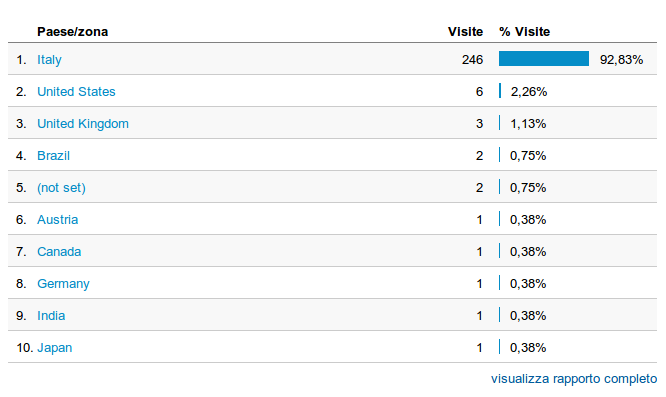
\includegraphics[width=0.95\textwidth,keepaspectratio=true]{img/googleAnalyticsPaesi}
	\centering
	\caption{Provenienza degli accessi al sito internet}%
	\label{fig:googleAnalyticsPaesi}%
\end{figure}
\begin{figure}[h!]%
	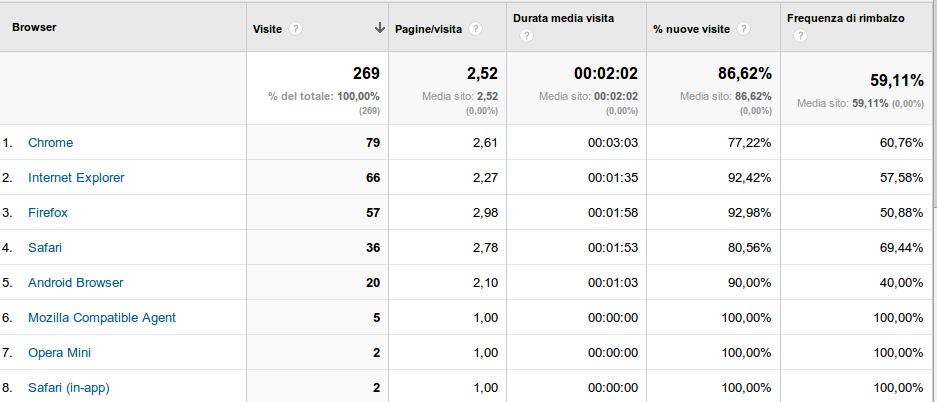
\includegraphics[width=0.95\textwidth,keepaspectratio=true]{img/googleAnalyticsBrowser}
	\centering
	\caption{Principali browser che accedono al sito}%
	\label{fig:googleAnalyticsBrowser}%
\end{figure}
\newpage
\section{Appendice C}
Appendice dei casi d'uso
\section{Appendice D}
Gli screenshot riportati sono stati prelevati dal risultato ottenuto dall'analisi effettuata tramite il servizio offerto dal sito \url{http://colorfilter.wickline.org/}. 
\par La mancanza delle immagini è dovuta dal fatto che il servizio non è riuscito ad analizzare i file di immagine presenti nello slider. Si fa inoltre presente che è stato 
analizzato il template del tema e non la versione finale.
\begin{figure}[h!]%
  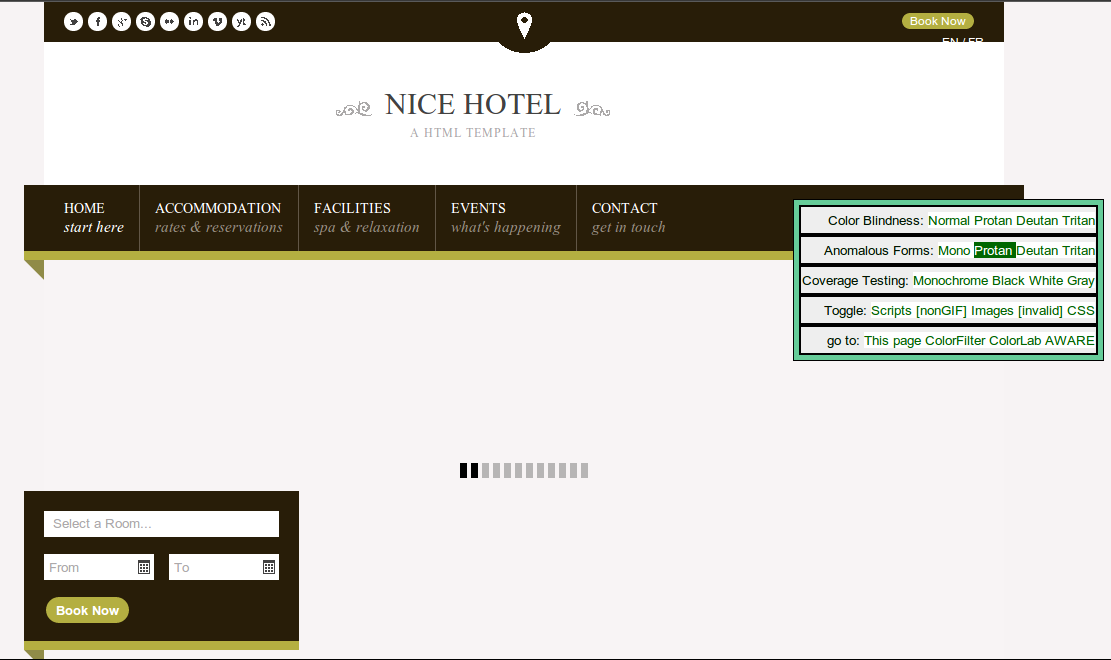
\includegraphics[width=0.95\textwidth,keepaspectratio=true]{img/daltonismoProtanopia}
  \centering
  \caption{Daltonismo: protanopia}%
  \label{fig:daltonismoProtanopia}%
\end{figure}

\begin{figure}[h!]%
  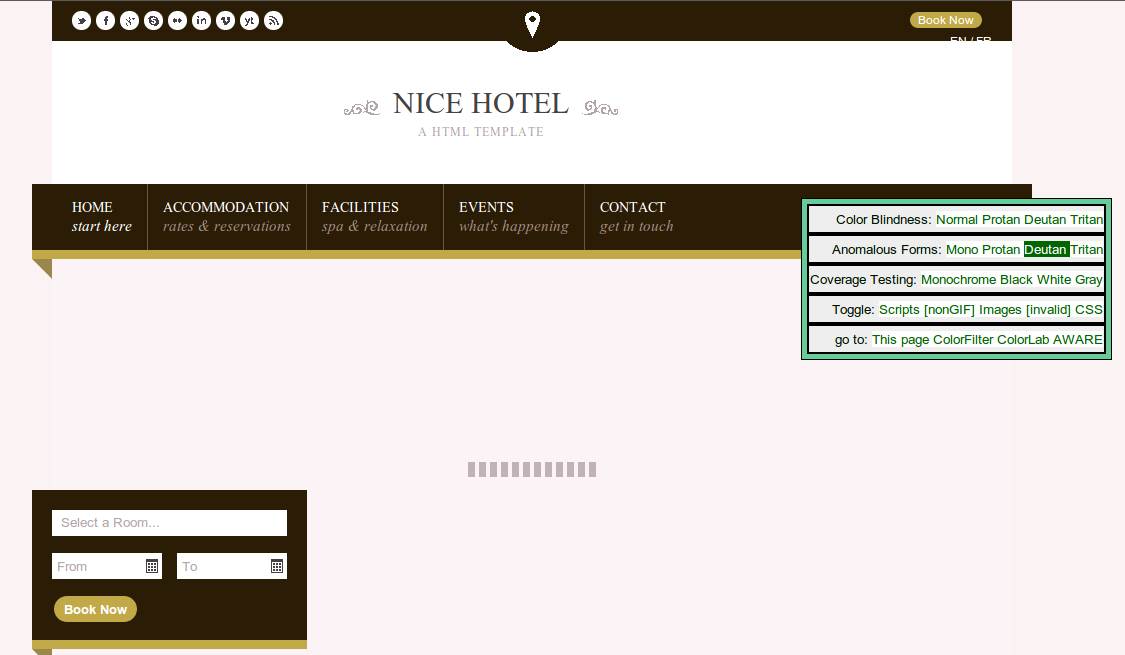
\includegraphics[width=0.95\textwidth,keepaspectratio=true]{img/daltonismoDeuteranopia}
  \centering
  \caption{Daltonismo: deuteranopia}%
  \label{fig:daltonismoDeuteranopia}%
\end{figure}

\begin{figure}[h!]%
  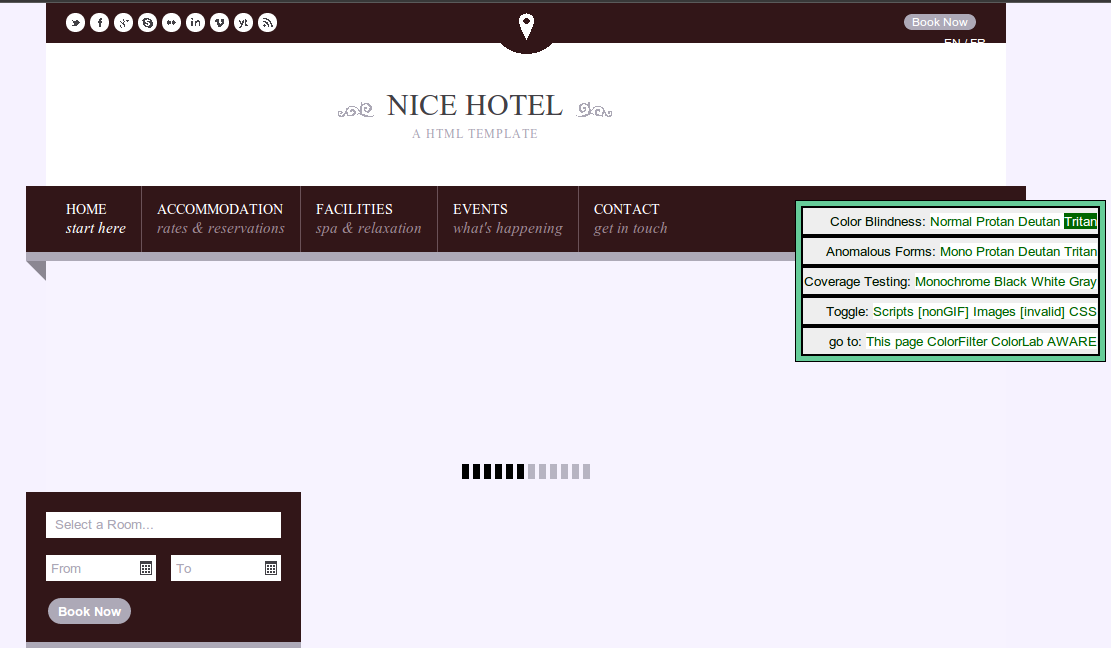
\includegraphics[width=0.95\textwidth,keepaspectratio=true]{img/daltonismoTritanopia}
  \centering
  \caption{Daltonismo: tritanopia}%
  \label{fig:daltonismoTritanopia}%
\end{figure}
Come si può notare dagli screenshot l'effetto di contrasto è comunque mantenuto non portando gravi anomalie che renderebbero il sito non navigabile dai daltonici. 
\\Sono state analizzate solamente le tre più comuni forme di daltonismo e soprattutto quelle legate maggiormente ai colori scelte nel tema.
\end{document}